
\begin{figure}[htbp]
\centering
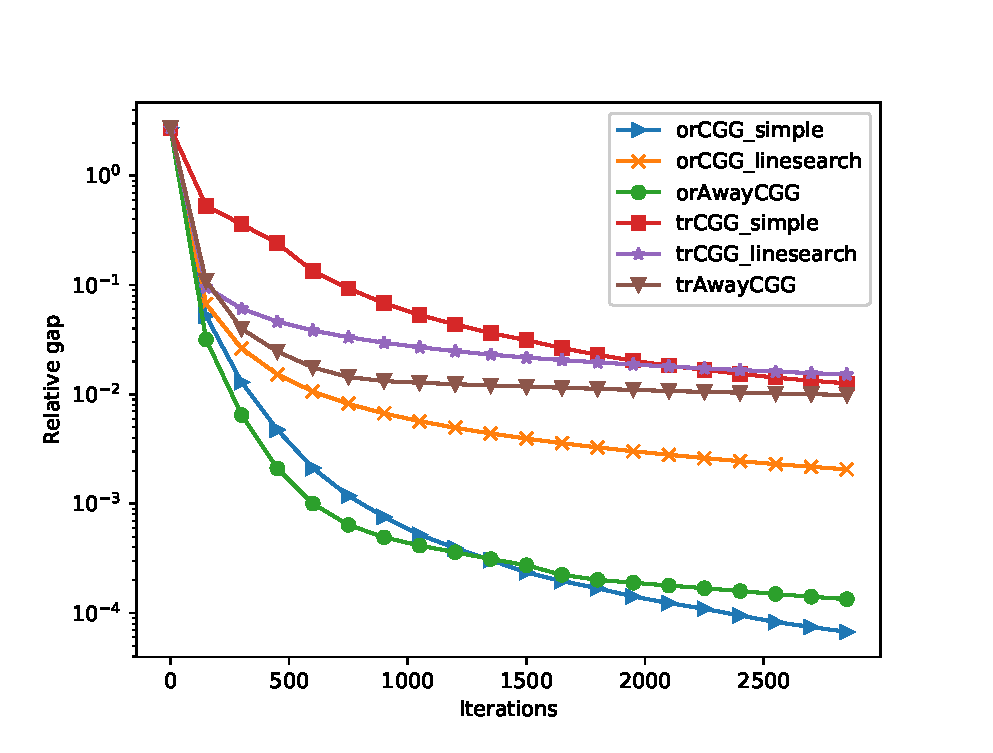
\includegraphics[height=7.2cm,width=9cm]{Images/Logistic_Iterations_vs_RelativeGap_7.eps}
\caption{Iteration-Gap figure for trend filtering with logistic loss $\sum_{i=1}^N \log \left( 1+\exp(-y_i\sigma x_i^T \beta) \right)$ and constraint $\|D^{(r)} \beta\|_1 \le \delta$, where $\beta\in \R^n$ with $N= 200$, $n = 400$, $r = 2$, $\delta= 0.8$ and $\sigma= 2.0e-02$. $y_1,...,y_N$ are i.i.d. samples generated from the distribution $\mathbb{P}(y_i = 1) = \frac{1}{1+\exp(-\sigma x_i^T \bar \beta)}, $ $\mathbb{P}(y_i = -1) = 1- \mathbb{P}(y_i = 1)$, where $\bar \beta$ is piecewise linear with 5 pieces and $\|D^{(r)} \bar \beta\|_1 = 1$.}
\label{Iteration-Gap7}
\end{figure}


\begin{figure}[htbp]
\centering
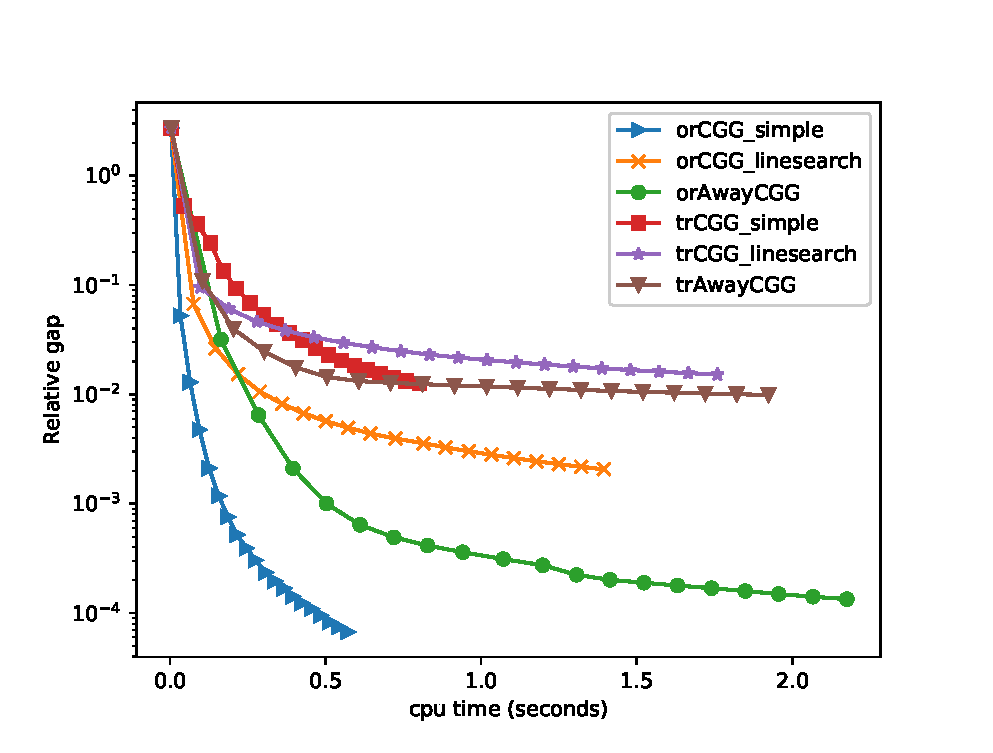
\includegraphics[height=7.2cm,width=9cm]{Images/Logistic_Time_vs_RelativeGap_7.eps}
\caption{Time-Gap figure for trend filtering with logistic loss $\sum_{i=1}^N \log \left( 1+\exp(-y_i\sigma x_i^T \beta) \right)$ and constraint $\|D^{(r)} \beta\|_1 \le \delta$, where $\beta\in \R^n$ with $N= 200$, $n = 400$, $r = 2$, $\delta= 0.8$ and $\sigma= 2.0e-02$. $y_1,...,y_N$ are i.i.d. samples generated from the distribution $\mathbb{P}(y_i = 1) = \frac{1}{1+\exp(-\sigma x_i^T \bar \beta)}, $ $\mathbb{P}(y_i = -1) = 1- \mathbb{P}(y_i = 1)$, where $\bar \beta$ is piecewise linear with 5 pieces and $\|D^{(r)} \bar \beta\|_1 = 1$. The time taken by CVXPY is 0.258274 seconds.}
\label{Time-Gap7}
\end{figure}

